\documentclass{infufrgs}

% Pacotes essenciais (a maioria já é carregada automaticamente pelo infufrgs.cls)
\usepackage[utf8]{inputenc}
\usepackage{framed}
\usepackage{amsmath}
\usepackage{graphicx} % Pacote necessário para inclusão de imagens

\colorlet{shadecolor}{orange!15}

\title{Relatório de Implementação e Análise: Algoritmo de Dijkstra e Heap $k$-ário}
% A classe infufrgs exige o formato \author{Sobrenome}{Nome}
\author{ROdrigues}{Juliana} 

\begin{document}
\maketitle

\chapter{Relatório de Análise Experimental}

\section{Introdução}
% Breve visão geral dos objetivos do projeto (implementação de um heap k-ário e do algoritmo de Dijkstra).
% Resumo do que o relatório irá abordar.

\section{Detalhes de Implementação}

\subsection{Representação do Grafo}
% Explicação da estrutura de lista de adjacências utilizada para suportar grafos esparsos com até ~24 milhões de vértices.

\subsection{Design do Heap $k$-ário}
% Detalhes sobre como o array do heap é gerenciado, como filhos/pais são calculados com base em k, e o array de mapeamento usado para buscas de vértices em O(1) durante a operação de update.

\subsection{Algoritmo de Dijkstra}
% Breve visão geral da integração do algoritmo com o heap.

\subsection{E/S e Convenções}
% Confirmação de que o programa aceita o formato DIMACS via stdin, lê source/dest através de argv, e lida corretamente com o caso limite "inf".

\section{Ambiente de Teste}

\subsection{Especificações de Hardware}
% CPU, RAM total e tipo de armazenamento (HDD/SSD, relevante para a E/S da Suite D).

\subsection{Stack de Software}
% Versão do SO, versão do compilador C++ (ex: GCC/Clang), e flags de otimização utilizadas (ex: -O3).

\subsection{Ferramentas de Benchmarking}
% Ambiente Python, métodos de medição de execução e scripts de geração de grafos.

\section{Resultados Experimentais e Análise}

\subsection{Ajuste de Parâmetros: Encontrando o Grau Ideal do Heap ($k$)}
% Objetivo: Determinar o valor de k que produz o melhor desempenho.

\begin{figure}[hbt!]
    \centering
    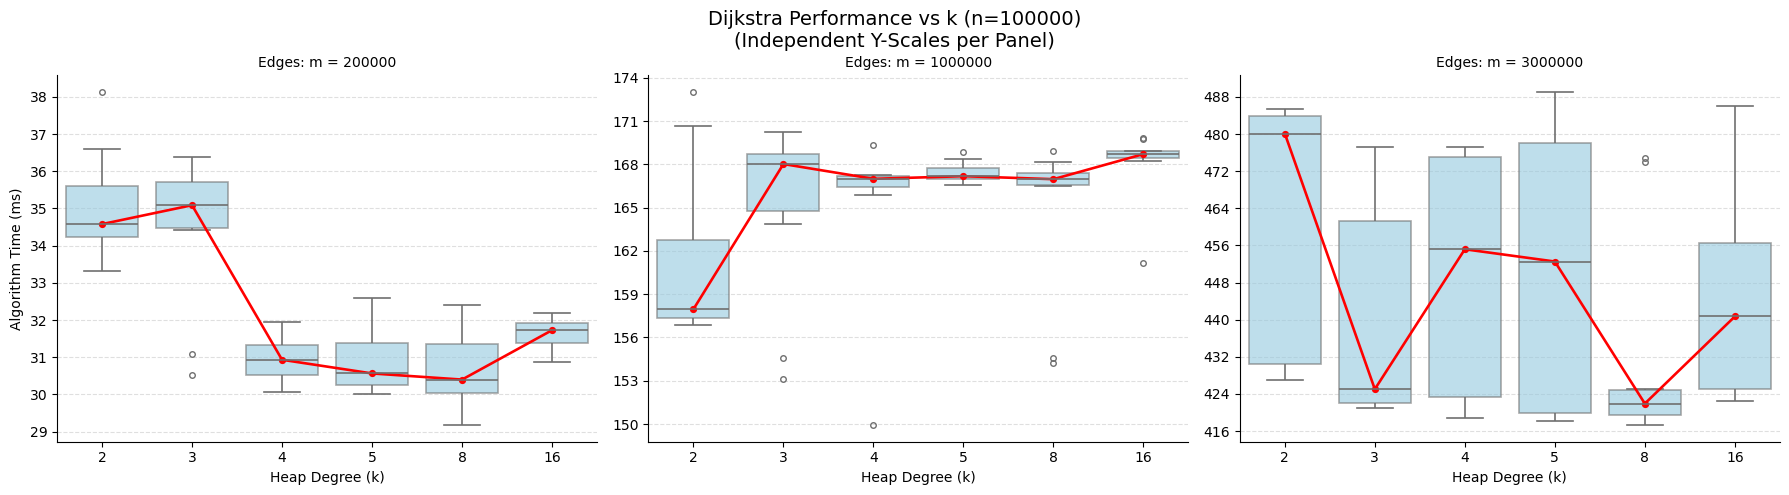
\includegraphics[width=0.8\textwidth]{Images/suiteA_graph1_performance_n100000.png}
    \caption{Tempo de execução em relação ao grau do heap $k$ para $n=100.000$.}
    \label{fig:perf_100k}
\end{figure}

\begin{figure}[hbt!]
    \centering
    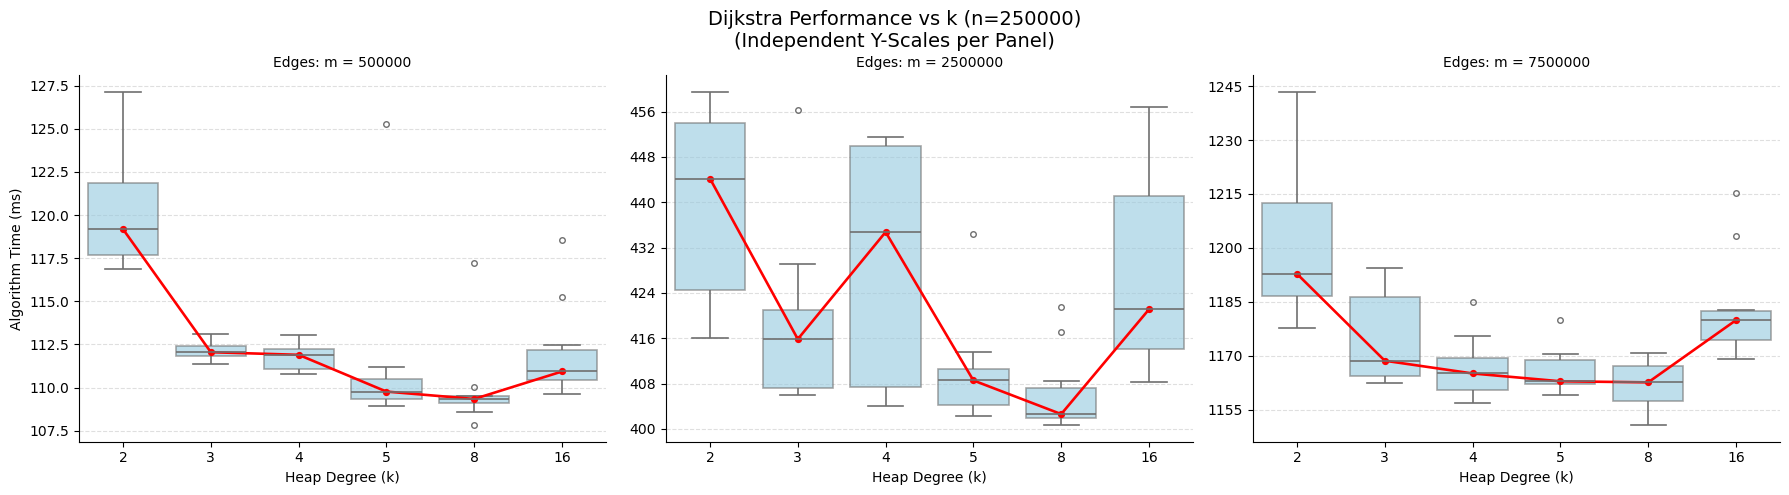
\includegraphics[width=0.8\textwidth]{Images/suiteA_graph1_performance_n250000.png}
    \caption{Tempo de execução em relação ao grau do heap $k$ para $n=250.000$.}
    \label{fig:perf_250k}
\end{figure}
% Descrição dos gráficos: Estes subgráficos facetados exibem o tempo de execução (eixo Y) em relação ao grau do heap k (eixo X) para várias densidades de grafos (m). Eles visualizam o trade-off em "curva U": valores pequenos de k sofrem com árvores profundas (update lento), enquanto valores grandes de k sofrem com nós largos (deletemin lento). O ponto mais baixo na linha de tendência da mediana vermelha comprova o k ótimo para a implementação.

\subsection{Validação da Complexidade do Heap}
% Objetivo: Verificar se o número de operações de sift respeita os limites teóricos (\le \log_k n').

\begin{figure}[hbt!]
    \centering
    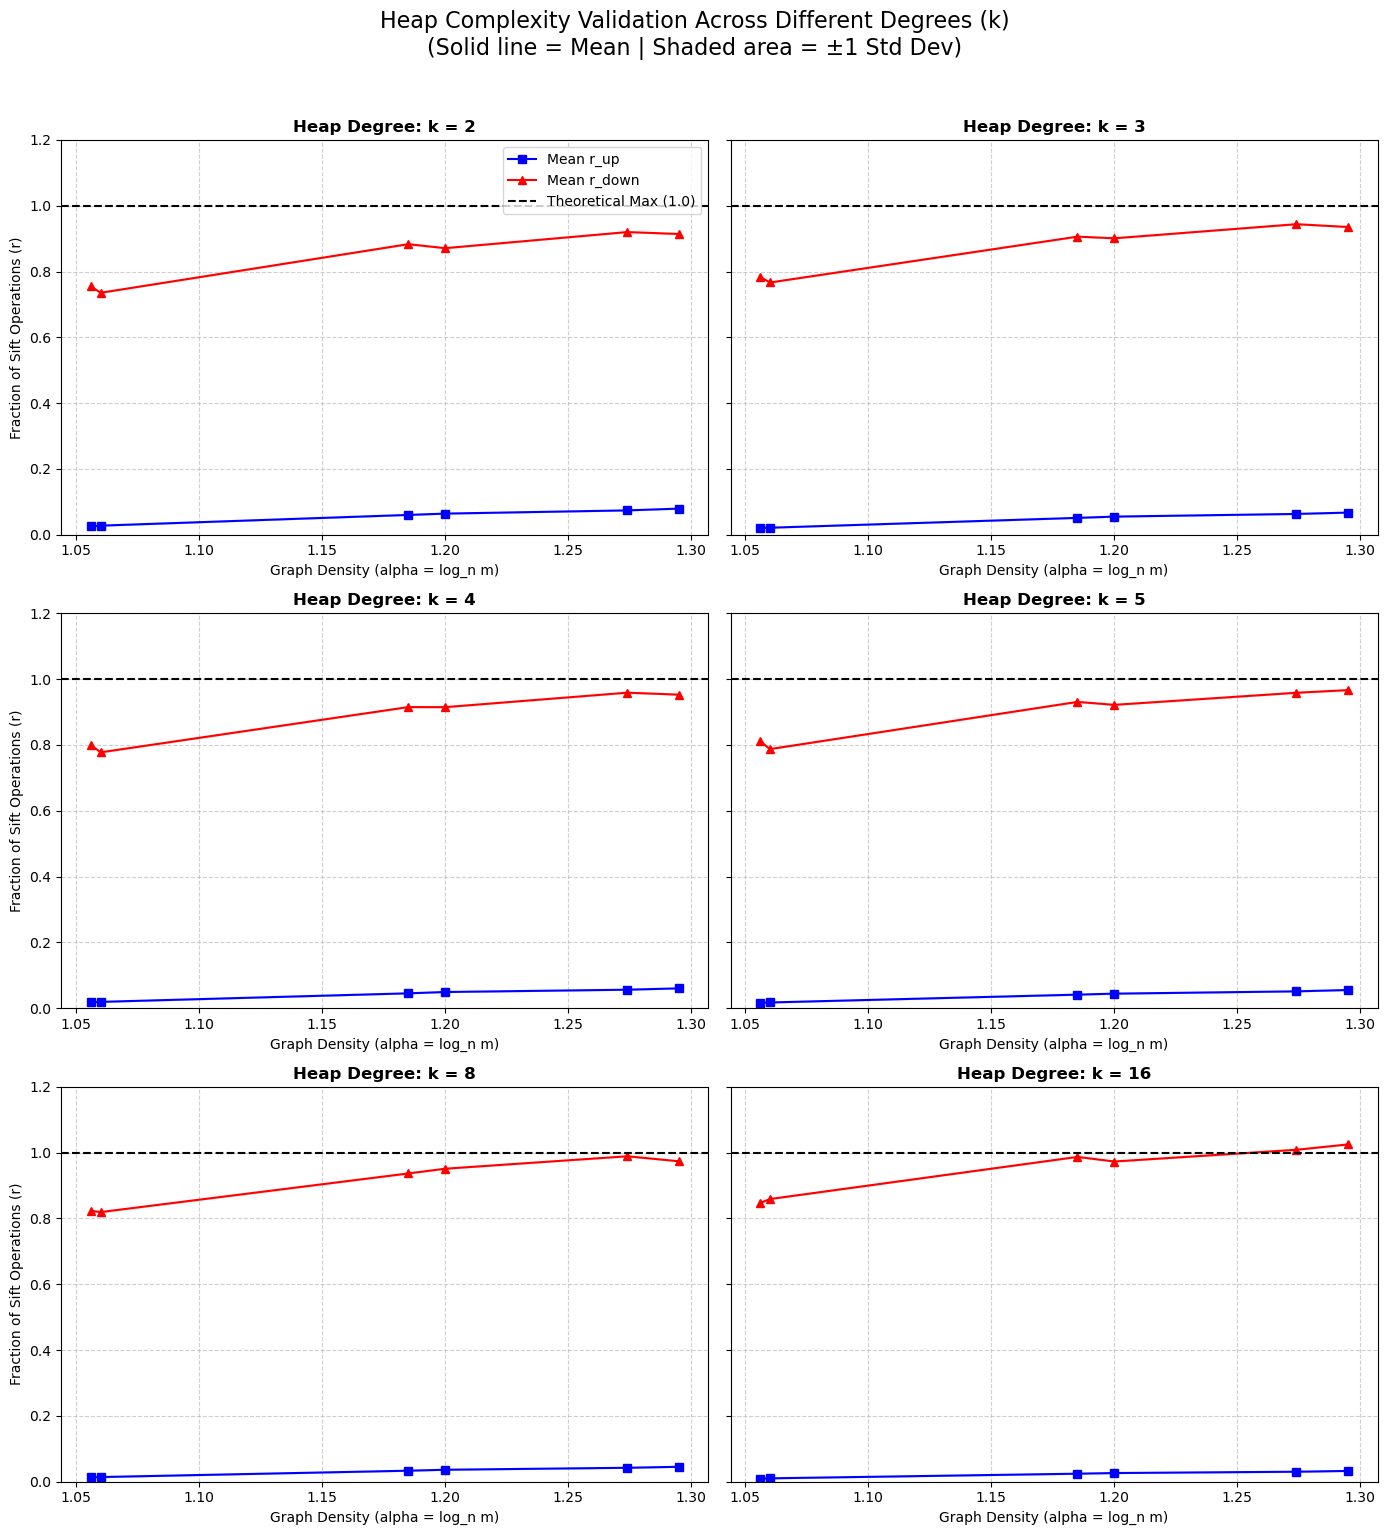
\includegraphics[width=\textwidth]{Images/suiteA_graph2_heap_complexity_combined.png}
    \caption{Fração das operações de sift em função da densidade do grafo para diferentes graus do heap ($k$).}
    \label{fig:heap_comp_combined}
\end{figure}
% Descrição dos gráficos: Esta grade de subgráficos mostra a fração das operações máximas possíveis de sift (r_up e r_down) no eixo Y contra a densidade do grafo (\alpha = \log_n m) no eixo X, organizados lado a lado para diferentes valores de k. A linha tracejada preta sólida em 1.0 representa o limite pessimista teórico. Os dados provam de forma consistente que as operações reais nunca ultrapassam este teto matemático e ilustram como a dinâmica interna das operações no heap se altera conforme a árvore se torna mais larga e rasa.

\subsection{Validação da Complexidade do Algoritmo: Operações de Atualização}
% Objetivo: Analisar a fração das operações de atualização como função de n e \alpha.

\begin{figure}[hbt!]
    \centering
    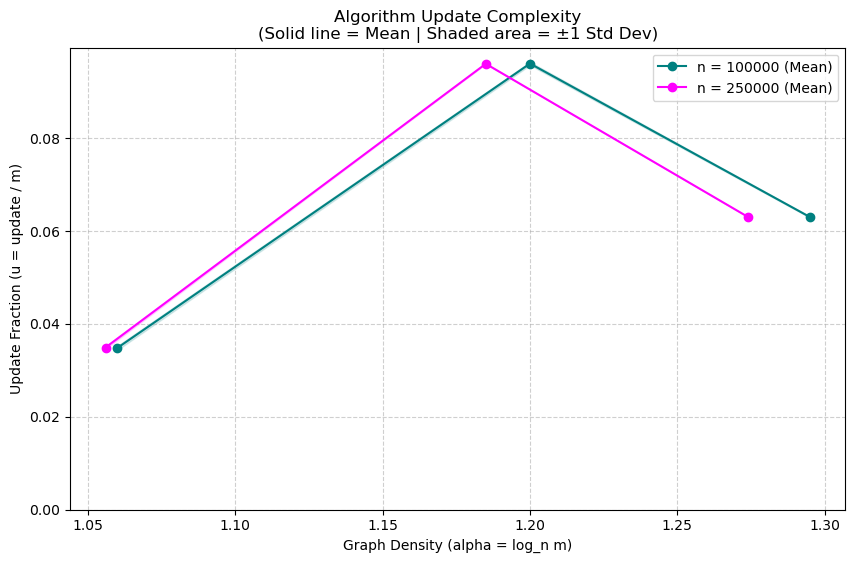
\includegraphics[width=0.8\textwidth]{Images/suiteA_graph3_update_complexity.png}
    \caption{Fração de atualizações $u$ em relação à densidade do grafo $\alpha$.}
    \label{fig:update_comp}
\end{figure}
% Descrição dos gráficos: Um gráfico de linha mostrando a fração de atualizações u = atualizações / m em diferentes densidades de grafos. Ele ilustra a frequência com que um caminho descoberto é de fato mais curto que um caminho conhecido anteriormente, demonstrando que, à medida que a densidade aumenta, a proporção de arestas que desencadeiam uma atualização estabiliza ou diminui.

\subsection{Análise do Caso Médio: Valor Esperado de Noshita}
% Objetivo: Comparar as contagens empíricas de atualização com a fórmula teórica de caso médio de Noshita.

\begin{figure}[hbt!]
    \centering
    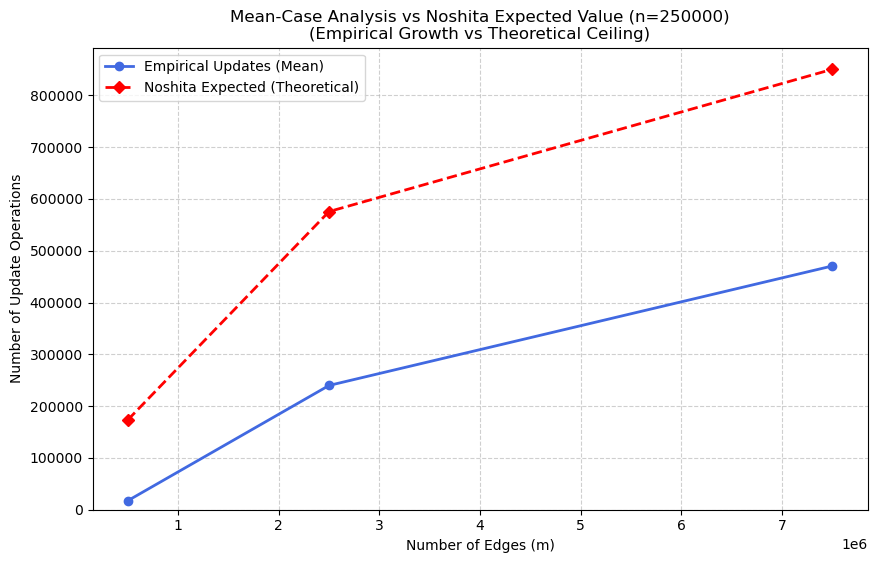
\includegraphics[width=0.8\textwidth]{Images/suiteA_graph4_mean_case_n250000.png}
    \caption{Análise de caso médio das atualizações vs. Valor Esperado de Noshita.}
    \label{fig:noshita}
\end{figure}

% Tabela com dados exportados do CSV demonstrando a variância microscópica.
\begin{table}[hbt!]
    \centering
    \begin{tabular}{|c|c|c|c|}
        \hline
        \textbf{m (Arestas)} & \textbf{Média Empírica (Updates)} & \textbf{Desvio Padrão} & \textbf{Noshita (Esperado)} \\ \hline
        % PREENCHER COM OS DADOS GERADOS PELO SCRIPT
        & & & \\ \hline
        & & & \\ \hline
    \end{tabular}
    \caption{Variância microscópica observada contra as previsões teóricas.}
    \label{tab:variance}
\end{table}
% Descrição dos gráficos: Um gráfico de linha comparando diretamente o número empírico de atualizações contra o valor esperado de Noshita à medida que o número de arestas (m) cresce. Valida visualmente que o comportamento do algoritmo no mundo real se alinha com a teoria matemática de caso médio.

\subsection{Avaliação do Escalonamento Assintótico}
% Objetivo: Avaliar o escalonamento do algoritmo de Dijkstra frente ao limite teórico O(m \log_k n + n \cdot k \log_k n).

\begin{figure}[hbt!]
    \centering
    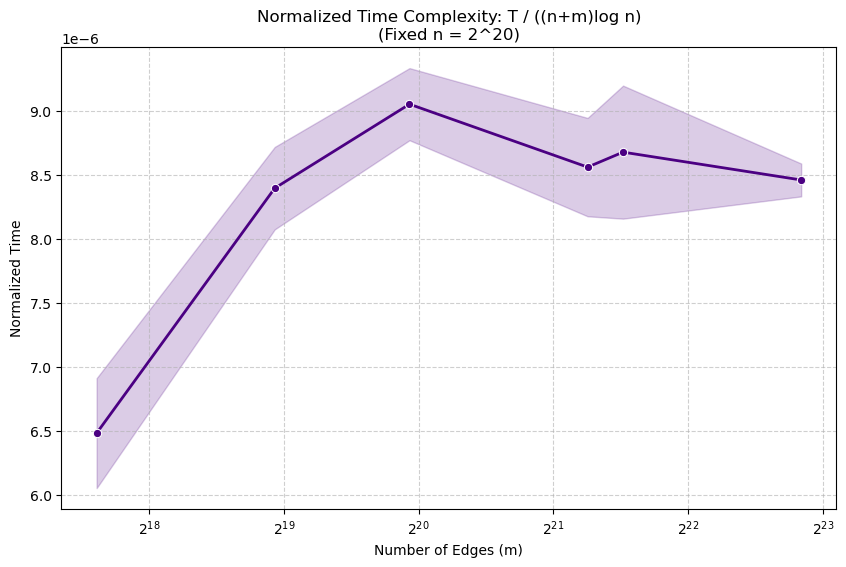
\includegraphics[width=0.8\textwidth]{Images/suiteB_normalized_complexity_varying_m.png}
    \caption{Complexidade de tempo normalizada variando o número de arestas ($m$).}
    \label{fig:norm_m}
\end{figure}

\begin{figure}[hbt!]
    \centering
    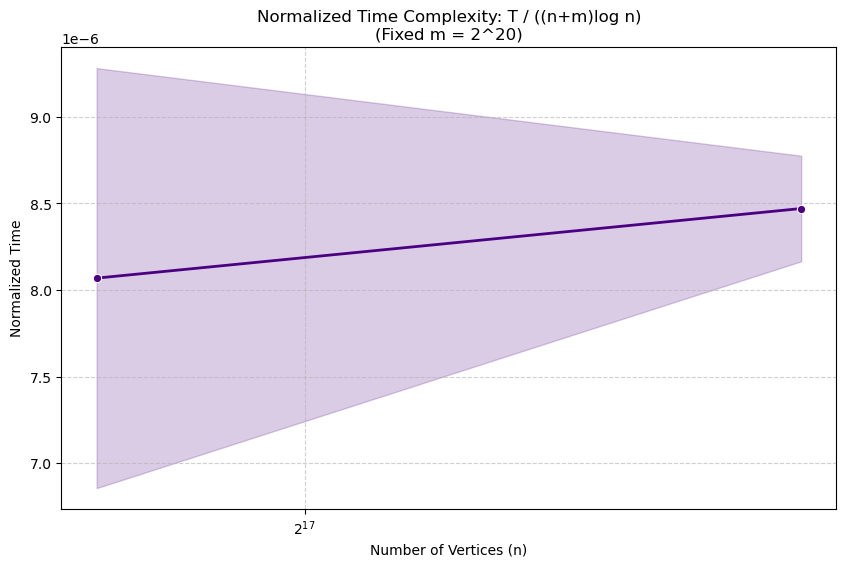
\includegraphics[width=0.8\textwidth]{Images/suiteC_normalized_complexity_varying_n.png}
    \caption{Complexidade de tempo normalizada variando o número de vértices ($n$).}
    \label{fig:norm_n}
\end{figure}
% Descrição dos gráficos: Estes gráficos mostram o tempo de execução normalizado contra a fórmula de complexidade teórica T / ((n+m)\log n). O fato de a linha plotada permanecer amplamente horizontal/plana à medida que n e m crescem exponencialmente prova que o algoritmo escala perfeitamente em conjunto com os limites teóricos.

\subsection{Análise de Regressão Linear Múltipla}
% Objetivo: Aplicar uma regressão linear T(n,m) \approx a \cdot n^b \cdot m^c ao conjunto de dados.

\begin{figure}[hbt!]
    \centering
    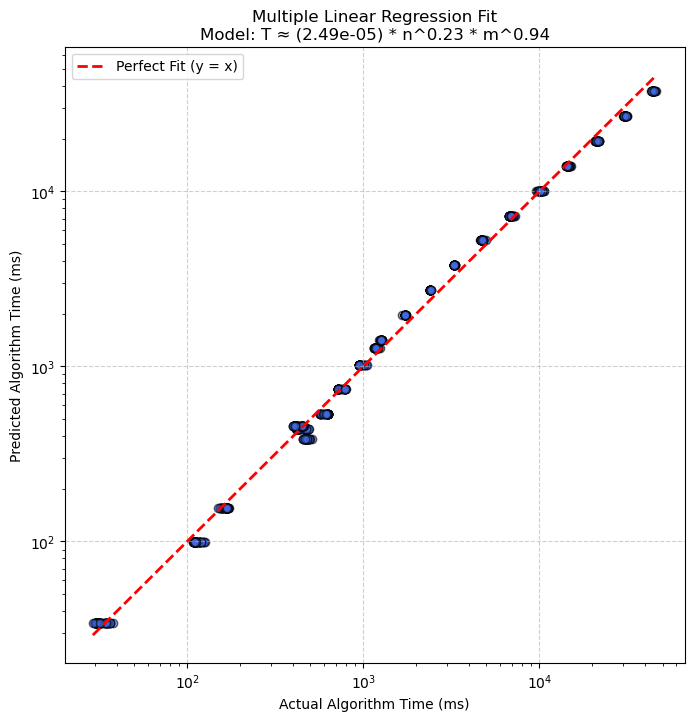
\includegraphics[width=0.8\textwidth]{Images/suiteR_actual_vs_predicted.png}
    \caption{Gráfico de dispersão Log-Log: Tempo Real vs. Previsto pelo Modelo.}
    \label{fig:reg_scatter}
\end{figure}

\begin{figure}[hbt!]
    \centering
    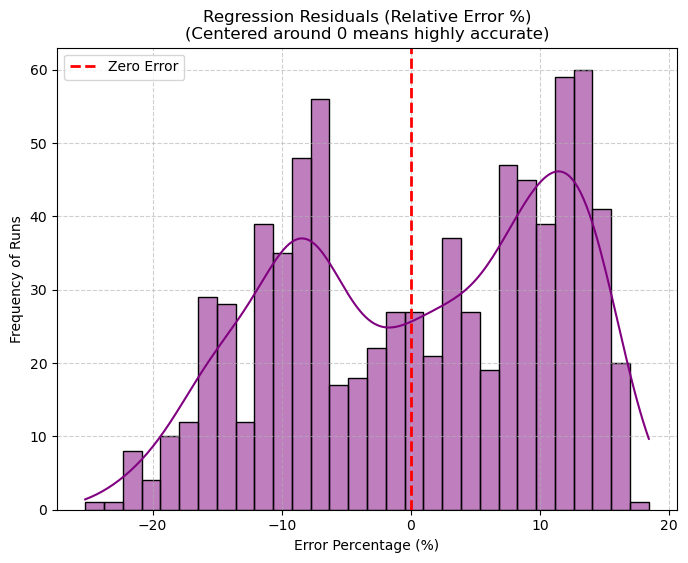
\includegraphics[width=0.8\textwidth]{Images/suiteR_residuals_error.png}
    \caption{Distribuição da porcentagem de erro relativo do modelo.}
    \label{fig:reg_error}
\end{figure}
% Descrição dos gráficos: O primeiro é um gráfico de dispersão log-log mapeando os tempos reais do algoritmo contra os tempos previstos pelo modelo de regressão, com uma linha vermelha representando um ajuste perfeito. O segundo é um histograma da porcentagem de erro relativo, demonstrando se a fórmula derivada tende a superestimar ou subestimar os tempos de execução.

\subsection{Desempenho no Mundo Real (Desafio DIMACS)}
% Objetivo: Analisar agendamento, tempo e consumo de memória em instâncias massivas do mundo real.

\begin{figure}[hbt!]
    \centering
    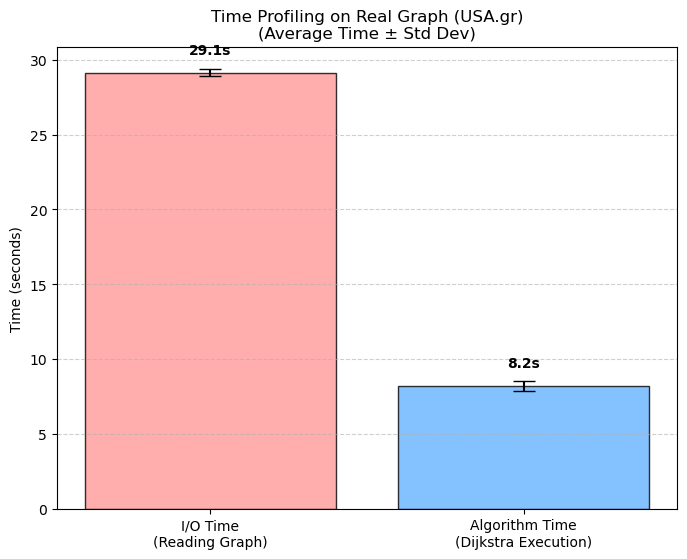
\includegraphics[width=0.8\textwidth]{Images/suiteD_time_profile_USA.gr.png}
    \caption{Perfil de tempo evidenciando o gargalo de E/S de disco.}
    \label{fig:dimacs_time}
\end{figure}

\begin{figure}[hbt!]
    \centering
    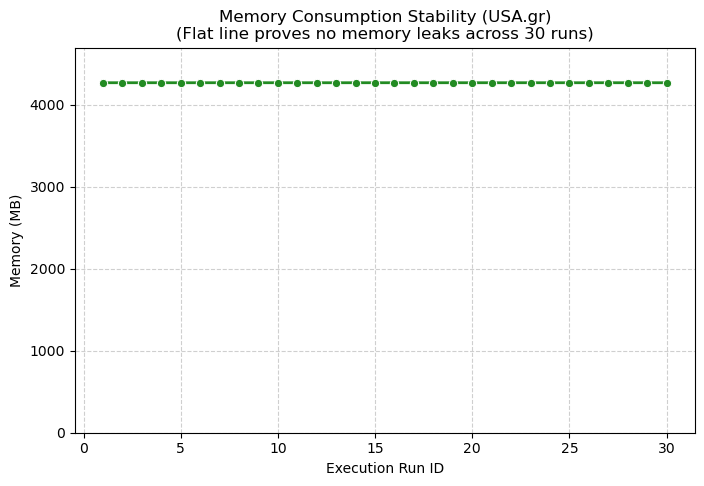
\includegraphics[width=0.8\textwidth]{Images/suiteD_memory_USA.gr.png}
    \caption{Consumo e estabilidade de RAM ao longo das execuções (Grafo USA).}
    \label{fig:dimacs_mem}
\end{figure}

\begin{figure}[hbt!]
    \centering
    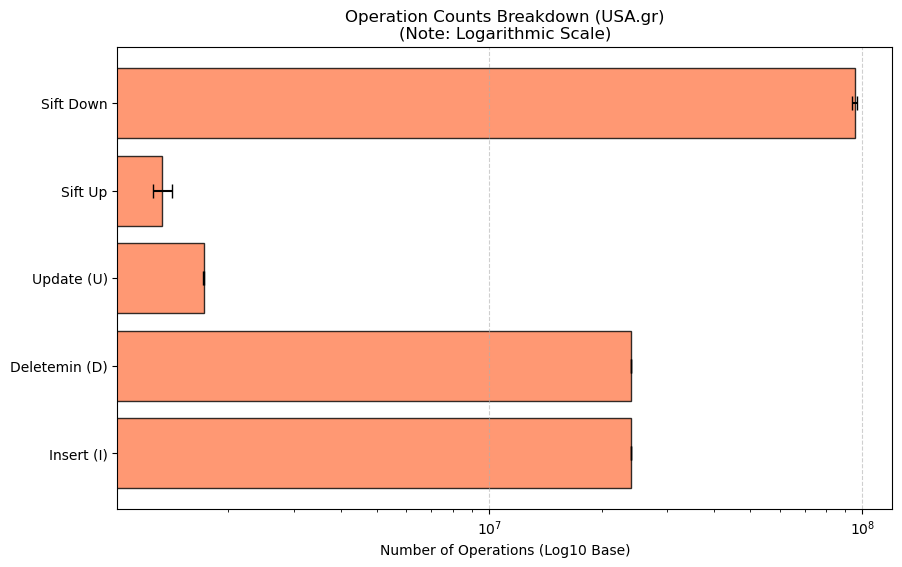
\includegraphics[width=0.8\textwidth]{Images/suiteD_operations_USA.gr.png}
    \caption{Detalhamento de operações executadas em rede rodoviária real.}
    \label{fig:dimacs_ops}
\end{figure}
% Descrição dos gráficos: 
% * Perfil de Tempo: Gráfico de barras revelando o enorme gargalo de E/S de Disco (leitura do arquivo de 24M de vértices) comparado ao tempo de execução altamente otimizado do algoritmo em si.
% * Memória: Gráfico de linha rastreando o uso de RAM ao longo de 30 execuções consecutivas, provando a complexidade espacial O(V+E) e confirmando visualmente a ausência de vazamentos de memória (memory leaks).
% * Operações: Gráfico de barras horizontais logarítmicas detalhando as contagens brutas das operações de Insert, Deletemin, Update, Sift_Up e Sift_Down desencadeadas ao atravessar toda a rede rodoviária dos Estados Unidos.

\section{Conclusão}
% Declaração final identificando o valor absoluto de k ideal descoberto.
% Confirmação de que a implementação respeitou com sucesso todos os limites teóricos pessimistas.
% Reflexões finais sobre a escalabilidade do algoritmo desde pequenos grafos sintéticos até redes rodoviárias de dimensão continental.

\end{document}